
\documentclass[11pt]{exam} % https://www.ctan.org/pkg/exam?lang=en

\usepackage[lmargin=1.in,rmargin=1.in,tmargin=1.in,bmargin=1in]{geometry}
\usepackage{setspace}
\usepackage[pdftex]{graphicx}
\usepackage{titling}
\usepackage[
	pdfauthor={Brian Weinstein},
	pdftitle={Homework 2},
	bookmarks=true,
	colorlinks=true,
	linkcolor=blue,
	urlcolor=blue,
	citecolor=blue,
	pdftex,
	linktocpage=true
	]{hyperref}
\usepackage[textsize=tiny]{todonotes}
\usepackage{float}
\setlength\parindent{0pt}


\qformat{\textbf{Problem \thequestion: \thequestiontitle}\quad \hfill}


\pagestyle{headandfoot}
\runningheadrule
\firstpageheader{}{}{}
\runningheader{\thetitle}{\theauthor}{\thedate}
\firstpagefooter{}{\thepage}{}
\runningfooter{}{\thepage}{}





\usepackage{xcolor}
\usepackage{adjustbox}
\usepackage{verbatim}
\definecolor{shadecolor}{rgb}{.9, .9, .9}

\newenvironment{code}%
   {\par\noindent\adjustbox{margin=1ex,bgcolor=shadecolor,margin=0ex \medskipamount}\bgroup\minipage\linewidth\verbatim}%
   {\endverbatim\endminipage\egroup}





\begin{document}


\title{STAT S4240 002, Homework 2}
\author{Brian Weinstein (bmw2148)}
\date{July 23, 2015}
\maketitle



\begin{questions}



\titledquestion{PCA}

\begin{parts}



\part Column means
\begin{code}
> apply(rawData, 2, mean)
       x1        x2        x3        x4        x5 
 6.049104 -8.277221  4.665532  7.914270 62.138753 
\end{code}
 
Row means
\begin{code}
> apply(rawData, 1, mean)
  [1]  -0.1277116  20.8162864  -8.8984358  25.5999204  -9.7472153
  [6]  64.0626702  22.0392371  23.3914888  31.7598224 -13.8680290
...
 [91]   1.2105932  21.2145724  -8.4896595  19.0639963  20.9767512
 [96]   3.5962333  22.3461063   0.7145014   6.3080005  64.8829556
\end{code}

The nonzero column means indicate that each variable isn't centered. In this context the row means are just the average of the coordinates for each observation. 
 
 
\part Empirical covariance matrix
\begin{code}
          x1         x2        x3        x4        x5
x1  72.96417  -83.90858  53.23708  120.1162  568.4105
x2 -83.90858  110.89101 -63.89570 -115.9430 -817.3388
x3  53.23708  -63.89570  39.60282   83.7386  445.2511
x4 120.11620 -115.94304  83.73860  232.1333  683.5587
x5 568.41046 -817.33884 445.25112  683.5587 6288.8569
\end{code}

The diagonal values tell us the variance of the variable indicated in the column (or equivalently, the row). The off-diagonal elements indicate the covariance between the two variables that intersect at that element.

\part The eigenvalues and eigenvectors of the empirical covariance matrix \texttt{sig}:
\begin{code}
> eigen(sig)
$values
[1] 6.557348e+03 1.868951e+02 2.038354e-01 9.775594e-04 9.373658e-05

$vectors
            [,1]       [,2]         [,3]        [,4]        [,5]
[1,]  0.09009603 -0.3247102 -0.383470773  0.82286709  0.24957150
[2,] -0.12797842  0.1364755  0.227047683 -0.11412319  0.94890526
[3,]  0.07028767 -0.1941349  0.894987159  0.37278501 -0.13191135
[4,]  0.11077853 -0.9008231 -0.019718518 -0.40719485  0.10024632
[5,]  0.97892389  0.1636064  0.002946326 -0.07133967  0.09921159
\end{code}

Since it's a symmetric matrix, \texttt{sig} has the same left eigenvectors as right eigenvectors.

\part The loadings are the eigenvectors (see part c). The scores are:
\begin{code}
> data%*%t(evecs)
               [,1]          [,2]         [,3]         [,4]        [,5]
  [1,]  -25.9233299  -50.96254603  -4.06557021  -8.91350845 -10.7755359
  [2,]   13.3064897   13.56908728   6.16049505   0.82185440   4.8621981
  [3,]  -37.6872799  -93.30323983  -1.02562352 -18.15040050 -16.3848300
...
 [98,]  -27.0931525  -38.88284377  -8.26671502  -5.26069573 -10.6527232
 [99,]  -13.1627026  -31.46409161  -1.20277265  -5.83681744  -5.6197025
[100,]   85.7232563  184.73133084  10.16179165  33.54024954  36.1560703
\end{code}

\part Proportion of variance explained

\begin{figure}[H]
	\centering
	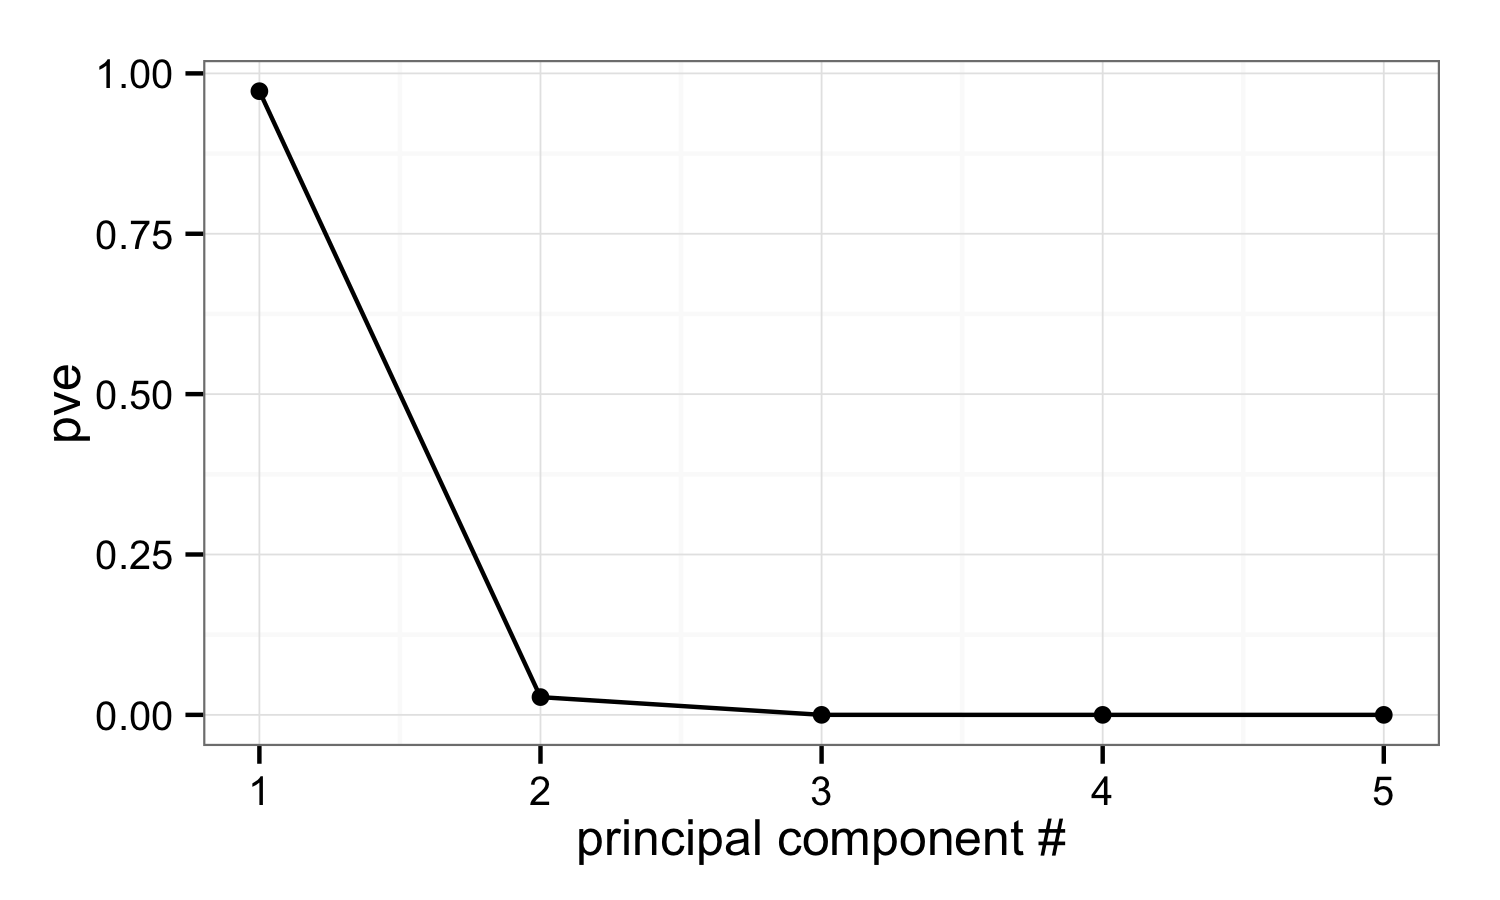
\includegraphics[width=5in]{1e.png}
	%\caption{}
	%\label{fig:figName}
\end{figure}

We only need one principal component. PC \#1 accounts for 97\% of the variance on its own, and including any additional PCs introduces more complexity than it's worth.

\part The scores for the new observations:

\begin{code}
> data2%*%t(evecs2)
            [,1]      [,2]      [,3]         [,4]        [,5]
[1,]  -6.0639533 -65.32443 16.218208 -20.96720620  -9.5868019
[2,]   0.6933977  25.72910 -7.634907   8.55181447   3.0468391
[3,]   2.0721371   1.97324  1.575201   0.03853202   0.9148939
[4,] -19.8318245 -61.16333  1.351568 -15.86750900 -14.2082956
[5,]  -8.6663467 -16.36235 -2.214696  -3.63623397  -5.2164795
\end{code}

where \texttt{data2} has been column centered.


\part Coordinates of the projections in the original space:

\begin{code}
          [,1]      [,2]      [,3]      [,4]      [,5]
[1,] 19.784390 -23.98670 -4.490318  2.926516  62.37239
[2,]  8.929318 -13.05966 15.636393 19.583344 148.49230
[3,] 12.023796 -16.96235  8.788414 17.696985 126.33419
[4,] 18.112666 -18.77458  3.584542 -7.331764  64.91650
[5,] 13.426490 -16.02315  9.502113  7.001699 108.06507
\end{code}

Euclidean distance from the original data points.
\begin{code}
[1] 28.18795
[1] 11.86206
[1] 1.822025
[1] 21.34198
[1] 6.733404
\end{code}


\part The error vectors are more or less orthogonal to the direction of the first principal component. This is because the error vectors are defined as the direction from the original points to their \textit{orthogonal projections} onto the reduced-dimension space, which, in this case, is primarily captured by the first PC. \todo{code isn't working. loadings are correct. errors start at or after calculating the scores}


\end{parts}




\titledquestion{PCA with Yale Faces B}


\begin{parts}

\part The matrix is 152 rows by 32,256 columns. Each row of the matrix is one photograph (38 subjects with 4 views each), and each column is a pixel in each image (originally 192 x 168).

\part 











\end{parts}


\titledquestion{\href{http://www-bcf.usc.edu/~gareth/ISL/}{James} 3.7.3}


\begin{parts}
\part
asdfasdf
\end{parts}


%\begin{figure}[H]
%	\centering
%	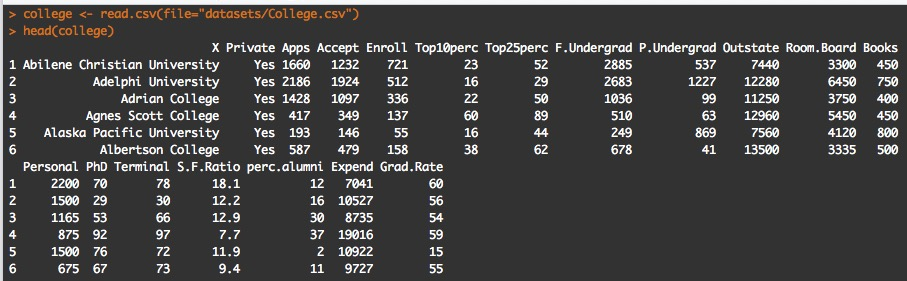
\includegraphics[width=6.5in]{8a.jpeg}
%	%\caption{}
%	%\label{fig:figName}
%\end{figure}


\end{questions}

\listoftodos

\end{document}